% !TeX root = main.tex
\chapter{Background}\label{chp:background}

\section{Audio visualisation principles}

Sound is temporal

Vision is spatio-temporal

Benefits:
- Screens are prevalent, so usually no extra equipment needed
- 

In a world of `big data', data visualization is becoming an increasing popular
subject. Visualization techniques have been applied to audio content for a
variety of applications including accessibility \citep{Ho-Ching2003}, browsing
large databases \citep{FontCorbera2010}, browsing small databases \citep{Yoo2011}
and musical training \citep{Ferguson2005} amonst others.

The development of good visualizations lies somewhere between science and art.
Tufte's seminal work on good practice \citep{Tufte2001} gives solid guidance on
creating elegent and unbiased visuals, and Wolfe and Horowitz \citep{Wolfe2004}
tell us which properties of vision are most critical for visual search.
However, putting these together in the context of audio requires a certain
amount of creativity.

This project focusses on `visualization of time-oriented data', a good overview
of which can be found in a Springer book of the same name \citep{Aigner2011}.
The rest of this section will look at examples of time-oriented visualization
of audio, grouped by the most common visualization techniques.

\subsection{Cross-modality}\label{sec:background-crossmodal}
%TODO What is cross-modality?
The ``bouba/kiki effect'' is a demonstration of cross-model mapping between vision and audition. It was originally
discovered in an experiment run by psychologist \citet{Koehler1929}. In the experiment, participants are shown two
abstract shapes and are asked to assign the name `bouba' to one of them, and `kiki' to the
%TODO Add original names
other\footnote{Originally the words XXX and YYY were used, but later changed}. To try out the experiment for yourself,
look at the shapes in Figure~\ref{fig:boubakiki} and see which shape you think best fits the name `bouba' and which
best fits `kiki'.

\begin{figure}[ht]
\centering
\begin{subfigure}{.5\textwidth}
  \centering
  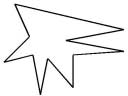
\includegraphics[width=0.7\linewidth]{figs/kiki.png}
  %\caption{Kiki}
  \label{fig:kiki}
\end{subfigure}%
\begin{subfigure}{.5\textwidth}
  \centering
  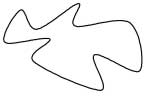
\includegraphics[width=0.7\linewidth]{figs/bouba.png}
  %\caption{Bouba}
  \label{fig:bouba}
\end{subfigure}
  \caption{Demonstration of the ``bouba/kiki effect'' \citep{Ramachandran2001}}
  \label{fig:boubakiki}
\end{figure}

K\"{o}hler found that the vast majority of participants chose to name the sharp, pointy shape `kiki' and the curvy,
rounded shape `bouba'. \citet{Ramachandran2001} found that that this effect holds for 95--98\% of the population. This
is an example of just one audio-visual mapping that is common amongst the population.
\citet{Spence2011} reviews a wide range of experiments from the world of psychology that attempt to find the inherint
cross-modal links in the human brain, including audio-visual mapping.
%\citep{Hubbard1996}

%These audio-visual associations are not just higher-level constructs that our
%concious brain creates, they affect the brain at the very lowest level even
%with only brief exposure to bimodal stimuli. Zangenehpour et. al.
%\citep{Zangenehpour2010} used a PET-CT scanner to measure blood flow in the
%brain during exposure to audio and visual stimuli. ``When presented with only
%the auditory or visual components of the bimodal stimuli, na\"{i}ve subjects
%showed only modality-specific cortical activation, as expected.  However,
%subjects who had previously been exposed to the audiovisual stimuli showed
%increased cerebral blood flow in the primary visual cortex when presented with
%sounds alone.''

Two test methods are used to discover these links -- `speeded' and `unspeeded'.  In `speeded' tests, participants are
asked to press a button as soon as they see/hear an audio-visual stimulus and their reaction time is measured. When the
reaction times are quicker, the stimuli are considered `congruent' (perceived to be similar). In `unspeeded' tests,
visual and audio stimuli are presented very quickly, one after the other, and participants are asked to choose which
one came first. When the just-noticeable difference (JND) time is higher, the stimuli are considered congruent, as they
are perceived to have merged into one entity.

\citet{Spence2011} found there to be strong evidence for six audio-visual mappings, which he grouped into three
categories:
{\singlespacing
\begin{itemize}
  \item Structural
  \begin{itemize}
    \item Loudness/brightness (louder=brighter)
  \end{itemize}
  \item Statistical
  \begin{itemize}
    \item Pitch/elevation (higher=higher)
    \item Pitch/size (higher=smaller)
    \item Loudness/size (louder=bigger)
  \end{itemize}
  \item Semantic
  \begin{itemize}
    \item Pitch/elevation (higher=higher)
    \item Pitch/spatial frequency (higher=higher)
  \end{itemize}
\end{itemize}
}

A recent experiment by \citet{Tsiros2014} attempted to measure audio-visual cross-modal link using audio visualization.
Three audio recordings were used -- a violin, recording of wind noise and impact sound event. For each, images were
manually created which used different combinations of audio-visual mappings (e.g. dissonance $\to$ texture
granularity). Participants were played an audio clip and shown an image and were asked whether they are similar or not,
and to what degree (on a scale of 0--100).  The experiment confirmed previous results which found strong links between
size/loudness and pitch/elevation, and weaker links between colour/pitch, granularity/dissonance, and colour
complexity/dissonance.

%Vision and audition are physiologically separate, but idential in many respects
%\citep{Tsiros2013}.

\section{Generative techniques}

\subsection{Waveform}

Benefits:
- Waveform is most recognisable visualisation
- Concept is very simple, easy to understand
- Simple to draw

Downsides:
- Displays limited information
- Mostly symetrical, wasting space
- audio wave-forms represent audio signal pressure over time and these signal representations are incredibly hard to interpret and use unless one is an audio-signal processing expert

\subsubsection{Colour mapping}\label{sec:background-colourmapping}
Mapping of data to colour can be separated into two methods -- pseudocolour and
false colour.

\paragraph{Pseudocolour}
This is a method of mapping a scalar value to a colour gradient
\citep{Moreland2009}. A commonly used example application of pseudocolour is
thermal imaging, where increasing temperature is mapped to a colour gradient of
blue$\to$green$\to$yellow$\to$orange$\to$red. The advantage of pseudocolour is
that it can emphasize small variations by using the full colour spectrum, or
make it easy to pick out highlights. However, as pseudocolour can only
represent one dimension, it does not make full use of the colour space.

Spectral waveform colouration has become a standard feature in DJ software,
first becoming popular after Serato Audio Research's `Scratch LIVE' program
introduced it.  DJs use the colour to distinguish between bass kicks, snares
and high-hats. Pseudocolour is used to enhanced the waveform, with spectral
centroid used as the input audio feature.

The same technique has been applied to other applications, notably on the audio
clip sharing website `Freesound' from Universitat Pompeu Fabra's Music
Technology Group\footnote{\url{http://blog.freesound.org/?p=10}, Bram de Jong,
  Music Technology Group, Universitat Pompeu Fabra, Barcelona}. The coloured
waveforms are used to help users quickly compare sound effect and music clips
on the website.

\paragraph{False colour}
This technique maps three values to a colour space, usually red/green/blue
(RGB). The advantage of this method is that it can use the full potential of
the colour available. However, it can be difficult to design/choose the three
values so that they map to colour in a coherent way that humans can easily
understand and interpret.

The technique of mapping audio frequencies to colour has been around since at
least 2000 when Tzanetakis and Cook introduced the concept of `Timbregrams',
which ``use color perception and the pattern recognition capabilities of the
human visual system to depict timbral and temporal information''
\citep{Tzanetakis2000}. Their implementation mapped the first three principal
components of a large feature vector to RGB colour space. According to the
authors, ``sound textures that are similar have similar colors''.

In 2005, Rice presented a similar idea, but used the colour to enhance
waveforms \citep{Rice2005}. The technique is not described in detail, but
generally it maps low/mid/high frequencies to blue/green/red. It is useful for
identifying timbrally distinct sounds and, with training, could be used to
identify certain sound effects. This system is currently marketed and licensed
as `Comparisonics' and has been integrated into DAW software from Magix and DJ
software from Native Instruments.

\begin{figure}[ht]
\centering
\begin{subfigure}{.5\textwidth}
  \centering
  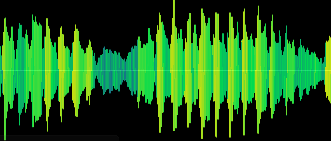
\includegraphics[width=\linewidth]{figs/freesound.png}
  \caption{Freesound (\url{freesound.com})}
  \label{fig:freesound}
\end{subfigure}%
\begin{subfigure}{.5\textwidth}
  \centering
  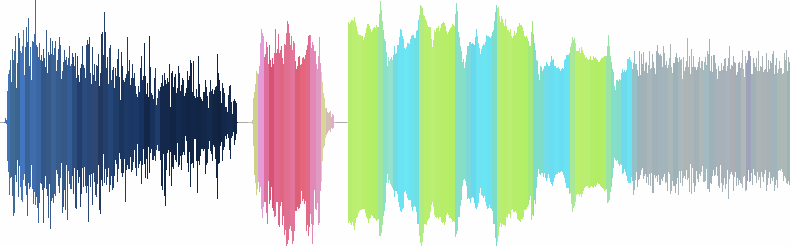
\includegraphics[width=\linewidth]{figs/rice.png}
  \caption{Comparisonics \citep{Rice2005}}
  \label{fig:rice}
\end{subfigure}
\caption{Examples of pseudocolour (\ref{fig:freesound}) and false colour
  (\ref{fig:rice}) applied to audio visualization}
\label{fig:colourvis}
\end{figure}

In 2007, the BBC created a system for visually representing recently-broadcast
radio material for navigation by the audience \citep{Mason2007}. It used three
basic features -- zero-crossing rate, its skewness and spectral rolloff --
which were each mapped to red, green and blue. Despite the arbitrarily-chosen
and simple features/mapping, the system is successful at indicating the
location of music within speech content, and highlighting low-bandwidth
material such as phone calls. The paper proposes in Section 7 that the system
could be used for assisted segmentation for podcast production.

Similar work was conducted at the BBC in 2013 by trainee Andrew Bonney who,
under the supervision of the author, looked into whether colour could represent
the sound of different people's voices. The result used median-filtered MFCCs
and gaussian mixture models, mapped to RGB colour space.
Figure~\ref{fig:bonney} shows an example of a recording with three speakers
(red/orange, blue and light/dark green).

\begin{figure}[ht]
  \centering
  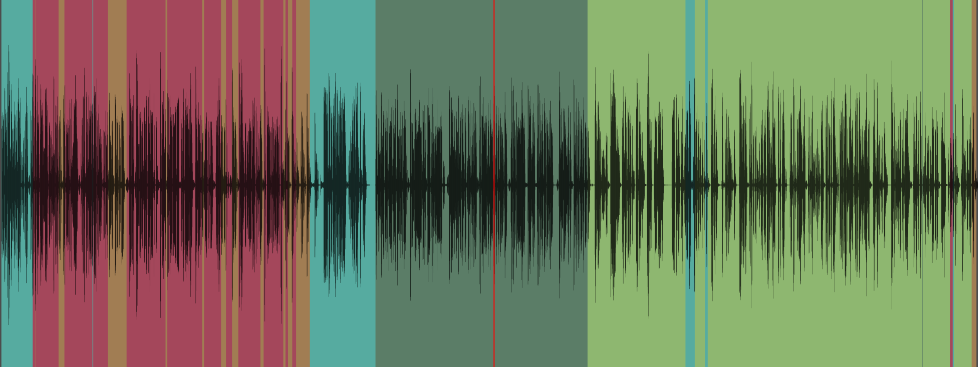
\includegraphics[width=0.95\linewidth]{figs/bonney.png}
  \caption{Speaker diarizartion through colour based on filtered MFCCs}
  \label{fig:bonney}
\end{figure}

False colour has also been used for navigating and summarizing extremely long
recordings. Towsey et. al. \citep{Towsey2014} mapped three spectral features to
RGB colour for visualizing almost a year of environmental recording.
Figure~\ref{fig:towsey} shows the recordings from March until October, with
each line representing one day. The visualization reveals the change in time of
the dawn and evening choruses throughout the year, amongst other things.

\begin{figure}[ht]
  \centering
  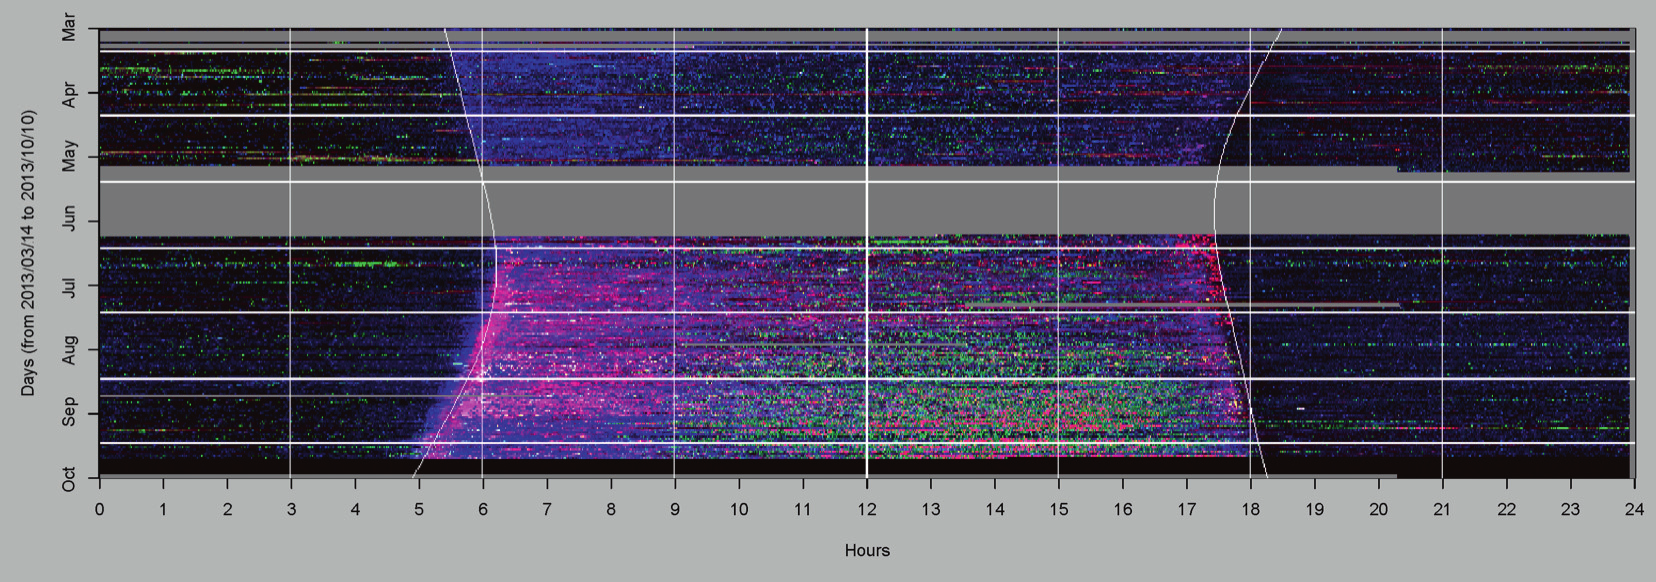
\includegraphics[width=0.95\linewidth]{figs/towsey.png}
  \caption{False colour visualization of environmental recordings, with each
    line representing one day. Missing data is grey.
    \citep{Towsey2014}}
  \label{fig:towsey}
\end{figure}

\subsubsection{Rescaling}
The `quintessence waveform' is a visualization developed by Loviscach
\citep{Loviscach2011} which attempts to address the problem of audio waveforms
not scaling well at different levels of zoom. It uses exteme pitch shifting so
that the character of the waveform is preserved at whatever scale the waveform
is viewed at (see Figure~\ref{fig:quint}). This approach works well for
monophonic material, but does not do so well with complex polyphonic material.

\begin{figure}[ht]
  \centering
  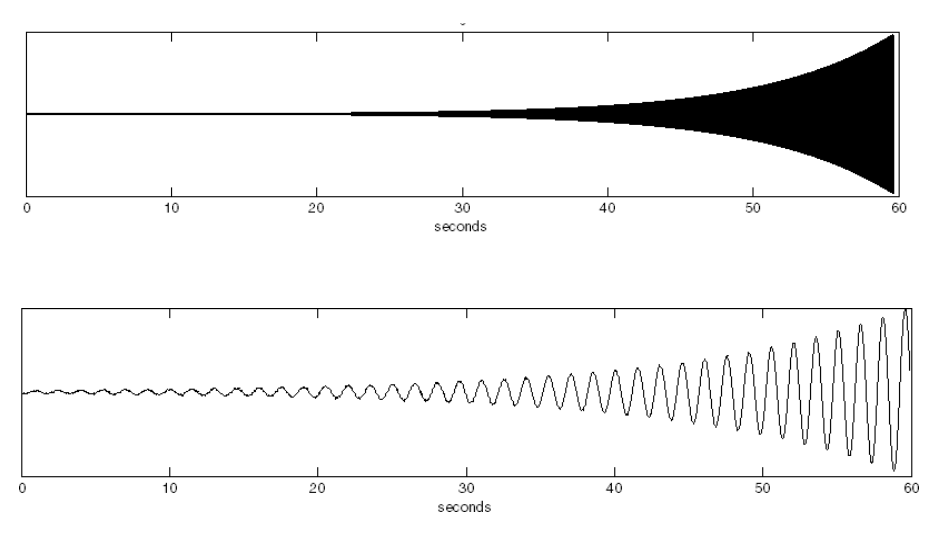
\includegraphics[width=0.95\linewidth]{figs/quint.png}
  \caption{Above: Normal waveform, below: quintessence waveform, source:
  \citep{Loviscach2011}}
  \label{fig:quint}
\end{figure}

\subsection{Spectrogram}

Not often used despite availablity

Pros
- High information density


Cons
- 

\subsubsection{Saliency mapping}
The University of Illinois have developed and evaluated enhanced spectrograms
for audio navigation \citep{Goudeseune2012,Lin2013}. The design was targeted
towards discovery of `acoustic events' and was implemented by creating a visual
saliency map of the spectrogram -- an image processing technique which attempts
to amplify the unique characteristics of the graphic.  Through the use of
custom browsing software called Timeliner (see Figure~\ref{fig:timeliner}), the
system was tested by recording how quickly users could find sound effects
hidden in long speech recordings. Although this task is not directly
applicable to radio production, the techniques used for the visualisation and
evaluation are of interest.

\begin{figure}[ht]
  \centering
  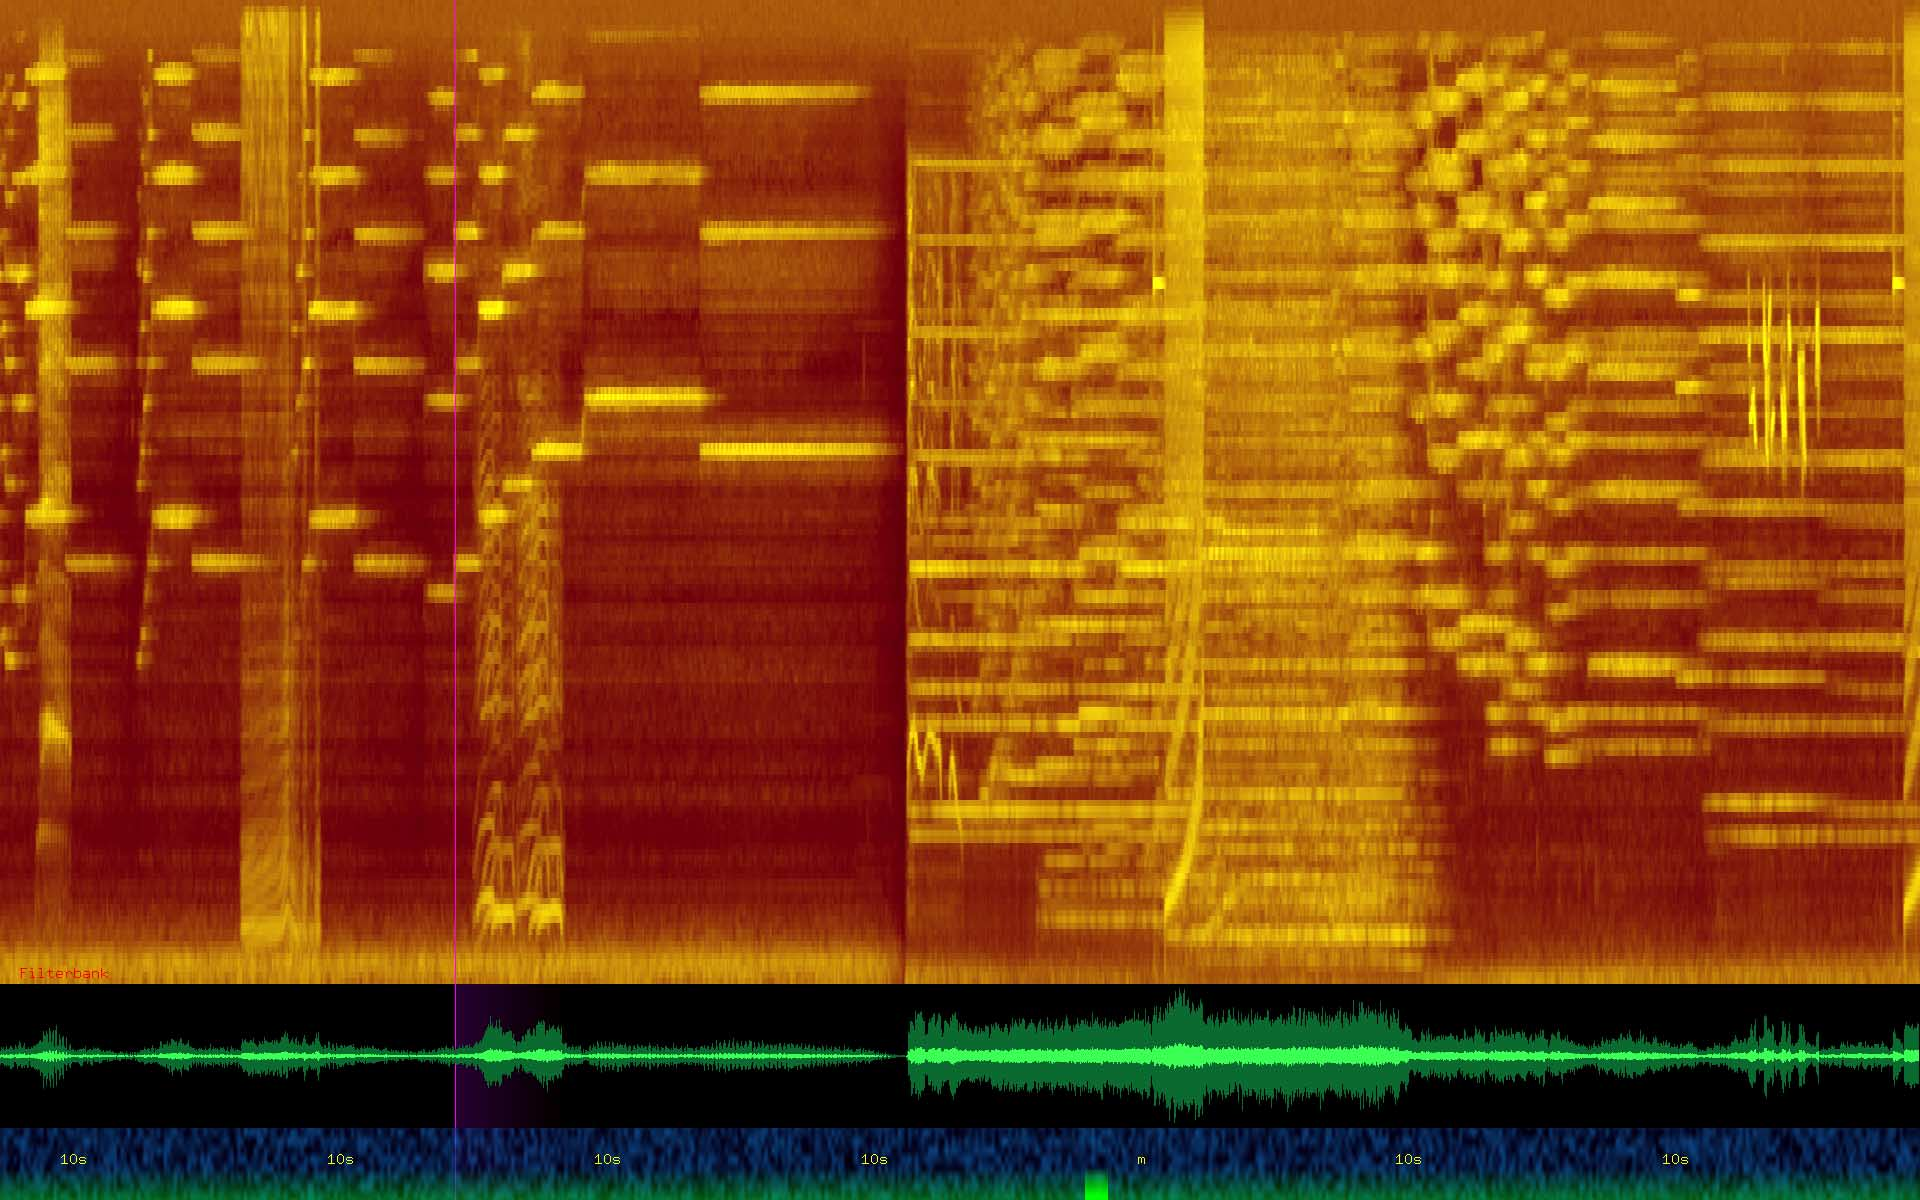
\includegraphics[width=0.95\linewidth]{figs/timeliner.png}
  \caption{User interface of `Timeliner', featuring a salience-mapped
    spectrogram, source: \citep{Goudeseune2012}}
  \label{fig:timeliner}
\end{figure}


\section{Semantic techniques}

\subsection{Segmentation}
Music structure
Speaker diarization

\subsection{Transcription}
Music transcription
Speech to text

\section{Alternatives}
Haptics

%======================================================================================================================

Academic research into audio analysis and audio interfaces tends to concentrate
on fully automated systems \citep{AngueraMiro2012}, navigation of large audio
collections \citep{FontCorbera2010} or navigation interfaces based on skimming
\citep{Arons1997} and scrolling \citep{Lee2007}. Although there are examples of
audio visualization from the world of academia, it is much more popular in the
context of art \citep{Armitage2012}, with excellent examples such as Quayola's
Form--Sound--Abstraction\footnote{\url{http://www.quayola.com/work/form-sound-abstraction/}}
work.

This section looks at three areas of literature from which the project will
draw upon -- extraction of meaningful audio properties, mapping these to a
visual representation, and the perceptual links between audition and vision.

\section{Feature extraction}\label{sec:litreviewfeats}
This section looks at audio features that could be used as part of an audio
visualization system. Firstly, two use cases that were previously identified as
being a common component of radio production are explored, before considering
methods of generating features for any use case.

\subsection{Speech/music discrimination}
Speech/music discrimination (SMD) is the process of segmenting audio content
into parts labelled by the categories speech and music. In general, SMD
classifiers use a collection of different features. This section lists the ones
that are used frequently or have recently been found to perform well.

\paragraph{RMS energy}
The root mean squared energy can be used also exclusively as an effective SMD
classifier, as demonstrated in \citep{Ericsson2009} and \citep{Panagiotakis2005}.
Commonly used statistics of RMS include low energy ratio
\citep{Liang2005,Ericsson2009,Saunders1996,Scheirer1997} and variance
\citep{Ericsson2009} (including normalised variance \citep{Panagiotakis2005} and
delta variance \citep{Carey1999}).

Low energy ratio (also known as `silent interval frequency' and `energy contour
dip') is a measure of the number of RMS energy frames that fall below a
threshold. It exploits the fact that speech has freqent silent gaps between
words, wheras music does not. The threshold can be set as a fixed value
\citep{Liang2005}, a function of a moving average \citep{Ericsson2009} or moving
peak value \citep{Saunders1996}.

Kacprzak and Zi\'{o}\l{}ko recently proposed a modified version of low energy
ratio called `minimum energy density' \citep{Kacprzak2013}. It is calculated by
normalizing over a $\sim$15 second window and finding the minimum of the
normalization function over a $\sim$1--3 second window. It has similar
performance to low energy ratio with a moving average threshold, but has fewer
parameters to set.

\paragraph{Zero-crossing rate} is the rate at which a signal crosses the time
axis, which is an easy-to-calculate measure for the spectral energy
distribution. Early work in SMD \citep{Saunders1996} identified that ``speech
signals produce a marked rise in the ZCR during periods of fricativity occuring
at the beginning and end of words'', wheras music does not. This causes a
bimodality which skews the ZCR distribition, which can be measured using the
third standardized moment (skewness). The variance of ZCR has also been found
to perform well for SMD \citep{Scheirer1997}.

ZCR also played a significant role in two steps of a five-step classifer
\citep{Panagiotakis2005}. During silent intervals the number of zero crossings
is null, so this was used to detect gaps between speech. The authors also noted
that ``RMS and ZCR are somewhat correlated for speech signals, while
essentially independent for music'', and so the product of RMS and ZCR was used
for the second classifier.

A review \citep{Carey1999} of features for SMD found ZCR to perform least well,
but did not consider the skewness, variance, or probability of null
zero-crossings.

\paragraph{MFCC}
Mel-frequency cepstral coefficients have long been the workhorse of audio
analysis, and they have been successfully used in SMD applications
\citep{Carey1999,Liang2005,Pikrakis2008,Pikrakis2006a,Sell2014,Wieser2014}.
Notably, their use has only been successful when used in combination with
strong machine learning systems, indicating that the relationship of MFCCs to
SMD labels is complex and non-linear. This would make it difficult to map to a
visual representation.

\paragraph{Chroma}
Use of chroma features work on the principle that the spectra of music is
aligned to the chromatic scale. Pikrakis et. al.
\citep{Pikrakis2006,Pikrakis2008} have successfully used `chromatic entropy' for
SMD applications. It takes sub-bands from a mel-scaled spectrum, aligned to the
chromatic scale, and calculates the entropy of the normalised spectral energy.

More recently, Sell \citep{Sell2014} has proposed two new chroma features, which
try to account for the fact that the chromagram varies greatly between
different pieces of music. Music tends to form strong, separated peaks on the
chromagram wheras speech has smoother mounds of energy. The new features
attempt to measure the peakiness of the chromagram. `Chromatic diff' subtracts
a shifted chroma vector from the original chroma vector and sums the energy. 
`Chroma high freq' performs an FFT on the chromagram and sums the high
frequency energy.

\paragraph{Continuous frequency activation}
Most of the above SMD features work well for segmenting speech-only/music-only
content. However, many fall down at detecting background music in speech.
Seyerlehner developed the continuous frequency activation (CFA) feature
\citep{Seyerlehner2007}, which works on the basis that music content has stable
harmonics, seen as horizontal lines on a spectrogram.

A moving average is subtracted from the FFT before it is binarized using a low
threshold value. For each bin, the proportion of active frames in an analysis
window is counted. The result is analysed with a peak picking algorithm and the
sum of the five largest peaks are used as the CFA. The result is a single
numeric value which quantifies the presence of steady frequency components.

In the original CFA paper, the feature was used to find music in television
content, but recently it has also been successfully applied to segmentaton of
radio recordings \citep{Wieser2014}.

\subsection{Speaker diarization}
Speaker diarization is the process of segmenting a speech recording by where
different people are talking. Review papers from 2006 \citep{Tranter2006} and
2012 \citep{AngueraMiro2012} show that the vast majority of systems are based on
clustering of MFCC or PLP features, which are low-dimensional representations
of speech. Rather than developing new features, the research is primarily
focussed on improvement of the clustering algorithms and pre-processing stages
such as Wiener filtering, speech activity detection and beamforming.

MFCC and PLP features are extremely effective when used in machine-based
classification systems, but from a human perception angle, the features do not
correlate well to what is heard.  Other features developed for automatic speech
recognition may also be useful in a speaker diarization system. For example,
spectral entropy \citep{Misra2004} is a measure of the peakiness of the spectrum
and is an effective feature in distinguishing between voiced and unvoiced
speech.

Friendland et. al. \citep{Friedland2009} proposed enhancing the standard MFCC
features with a set of long-term features representing prosody (the rhythm and
intonation of speech). 52 candidate features were ranked using feature
selection, which showed that ``the median and mean fundamental frequency are
the best features, following by high formants (F4, F5)''. Inclusion of the
top ten prosodic features improved the speaker diarization system by 24\%.

\subsection{Feature generation}\label{sec:litreviewgeneration}
Traditionally, audio features were developed by hand for specific tasks. This
was usually done by attempting to write an algorithm that calculated the
properties of the sound that humans used to distinuish the categories in
question. More recently, fuelled by an ever-increasing availability of
computing power, research has had a much greater focus on automating
this process.

\paragraph{Feature selection/extraction}
Feature selection and extraction are methods of reducing the dimensionality of
a feature vector, either by choosing a combination of vector components that
best describe the content (selection), or by translating the feature vector to
a smaller vector while retaining as much information as possible (extraction).

This process can be unsupervised where only the feature data is known (such as
with principal component analysis), or supervised where the feature data has
corresponding labels (such as with linear discriminant analysis).

Canonical correaltion analysis (CCA) has been used to reduce the dimensions of
features for speaker diarization \citep{Chaudhuri2009} and phonetic labelling
\citep{Arora2014}, amongst other things. It is able to efficiently map features
to a subspace and can be used with the kernel trick (known as KCCA) to support
non-linear mappings. In the case of speaker clustering, ``CCA-based algorithms
consistently provide better performance than standard PCA-based clustering
methods'' \citep{Chaudhuri2009}.

\paragraph{Feature learning}
The above methods of reducing dimensionality are based on a relatively short
information-rich feature vector that it suitable for the target application.
More recent research on feature development is focussed on automated learning
of features using large labelled datasets.

Deep learning is an increasingly popular method of learning features based on
neural networks with large numbers (tens or hundreds) of hidden units. This
line of research has been enabled by the increasing availability of large
amount of processing power. When done properly, deep learning can produce the
state-of-the-art in audio features, outperforming even the best hand-crafted
features \citep{Hamel2010,Sigtia2014}.

Such an approach requires a high-quality and very large labelled dataset, on
which the success of the process depends. The nature of neural networks means
that it is very difficult to interpret what the resulting features represent
which isn't an issue when used as the input to a machine learning system, but
would make it very difficult to map to a visualization. The objective of the
deep learning process is to minimise a cost function rather than to maximise
the link to human perception.
